\documentclass[twocolumn,UTF8]{ctexart}
\usepackage[a4paper,margin=1.8cm]{geometry}
\usepackage{amsmath,amssymb}
\usepackage{graphicx}
\usepackage{booktabs}
\usepackage{caption}
\usepackage{hyperref}
\usepackage{float}
\usepackage{xcolor}

\setlength{\columnsep}{0.7cm}
\captionsetup{font=small}
\hypersetup{colorlinks=true, linkcolor=blue, citecolor=blue, urlcolor=blue}

\title{\textbf{机器学习驱动的 A 股多因子 Alpha 挖掘与回测研究}\\
\large Machine Learning Alpha Research for A-Share Equity Returns}
\author{浙江大学统计学本科生量化研究项目}
\date{2026年5月}

\begin{document}
\maketitle

\begin{abstract}
本文构建了一个基于 AKShare 公开 A 股日频数据的 Machine Learning Alpha Research 框架。研究流程覆盖 AKShare 数据下载、股票池过滤、未来收益标签构造、36 个价量 Alpha 因子、横截面去极值与标准化、单因子 IC/RankIC 分析、Random Forest、XGBoost、LightGBM 与 PyTorch MLP 模型训练，以及样本外预测、分组回测、交易成本敏感性和稳健性分析。本次实验使用 2021--2024 年 98 只有效 A 股股票的前复权日频数据。结果显示，模型样本外 RankIC 为弱正，但在 2024 年测试区间内并未稳定跑赢等权股票池基准。本文强调严谨研究流程和风险披露，不将结果表述为稳定盈利策略。
\end{abstract}

\section{Introduction}
机器学习 Alpha Research 的核心目标，是在低信噪比的金融横截面数据中寻找可检验、可复现、可解释的弱预测信号。相比单纯报告一条收益曲线，一个合格的量化研究流程更应关注数据口径、标签定义、因子生成时点、样本外验证、交易成本和稳健性。

本文围绕如下问题展开：机器学习模型能否基于 A 股日频价量因子提取具有样本外稳定性的 Alpha 信号，并在考虑交易成本后改善横截面收益预测与组合回测表现？方法上，本文不直接追求复杂 Transformer，而是从 Random Forest、XGBoost、LightGBM 与简单 MLP 出发，因为日频 tabular alpha 数据通常噪声较高、维度有限，GBDT 类模型往往是更合理的强 baseline \cite{gu2020empirical,chen2016xgboost,ke2017lightgbm}。

\section{Data and Preprocessing}
数据来自 AKShare 公开 A 股日频接口。本次运行使用内置中等规模 A 股候选股票池 100 只，下载 2021-01-04 至 2024-12-31 的前复权日频行情。最终 98 只股票下载成功，共 94,382 行数据，字段包括 date、code、open、high、low、close、volume、amount、turnover\_rate 和由 outstanding shares 近似计算的 market\_cap。

由于 AKShare 实时股票列表接口在本环境中不稳定，本文使用固定示例股票池并逐只下载历史数据。固定股票池可能带来股票池选择偏差或幸存者偏差，因此本文不把结果表述为完整全 A 实证结论。股票池过滤包括价格、成交量、成交额、最短历史长度和缺失比例检查。真实生产研究还应加入 ST 状态、上市天数、停牌、涨跌停、行业分类和可交易性约束。

\section{Label Definition}
主标签为未来 5 日收益：
\begin{equation}
y_{5d,t}=\frac{Open_{t+6}}{Open_{t+1}}-1.
\end{equation}
含义是在 $t$ 日收盘后生成因子和模型分数，于 $t+1$ 日开盘买入，持有 5 个交易日，于 $t+6$ 日开盘卖出。项目同时生成 $y_{1d}$、$y_{5d}$、$y_{10d}$ 与 $y_{20d}$，用于持有期稳健性分析。

\section{Alpha Factor Construction}
本文构造 36 个基础价量因子，覆盖七类经济含义：动量/反转、波动率、流动性、量价关系、成交活跃度变化、价格位置和风险调整收益。所有 rolling 计算均按股票代码分组，且只使用 $t$ 日及以前的信息。例如，短期反转由 ret\_1、ret\_3、ret\_5 刻画；波动风险由 rolling return volatility 和 high-low amplitude 刻画；量价关系由 rolling correlation between return and volume/amount 刻画；成交活跃度变化由 5 日均值相对 20 日均值刻画。

\section{Factor Preprocessing}
每个交易日内对每个因子独立执行 1\%/99\% 分位数缩尾，随后做横截面 z-score。代码保留市值中性化接口：
\begin{equation}
factor_i=\alpha+\beta\log(MarketCap_i)+\epsilon_i.
\end{equation}
但本次 AKShare 运行不启用市值中性化，因为前复权价格与 outstanding shares 近似得到的 market\_cap 并不是严格的 point-in-time 风险模型口径。缺失值不会简单填 0；模型训练前删除缺失标签或缺失完整特征向量的样本。

\section{Single Factor Analysis}
单因子评价包括 Pearson IC、Spearman RankIC、ICIR、t-stat、胜率、因子相关矩阵和分组收益。RankIC 更关注横截面排序能力，因此比单纯 MSE 更贴近选股任务。本次 AKShare 运行中，RankIC 较高的因子包括 turnover\_mean\_20 等成交活跃度类指标。

\begin{figure}[H]
\centering
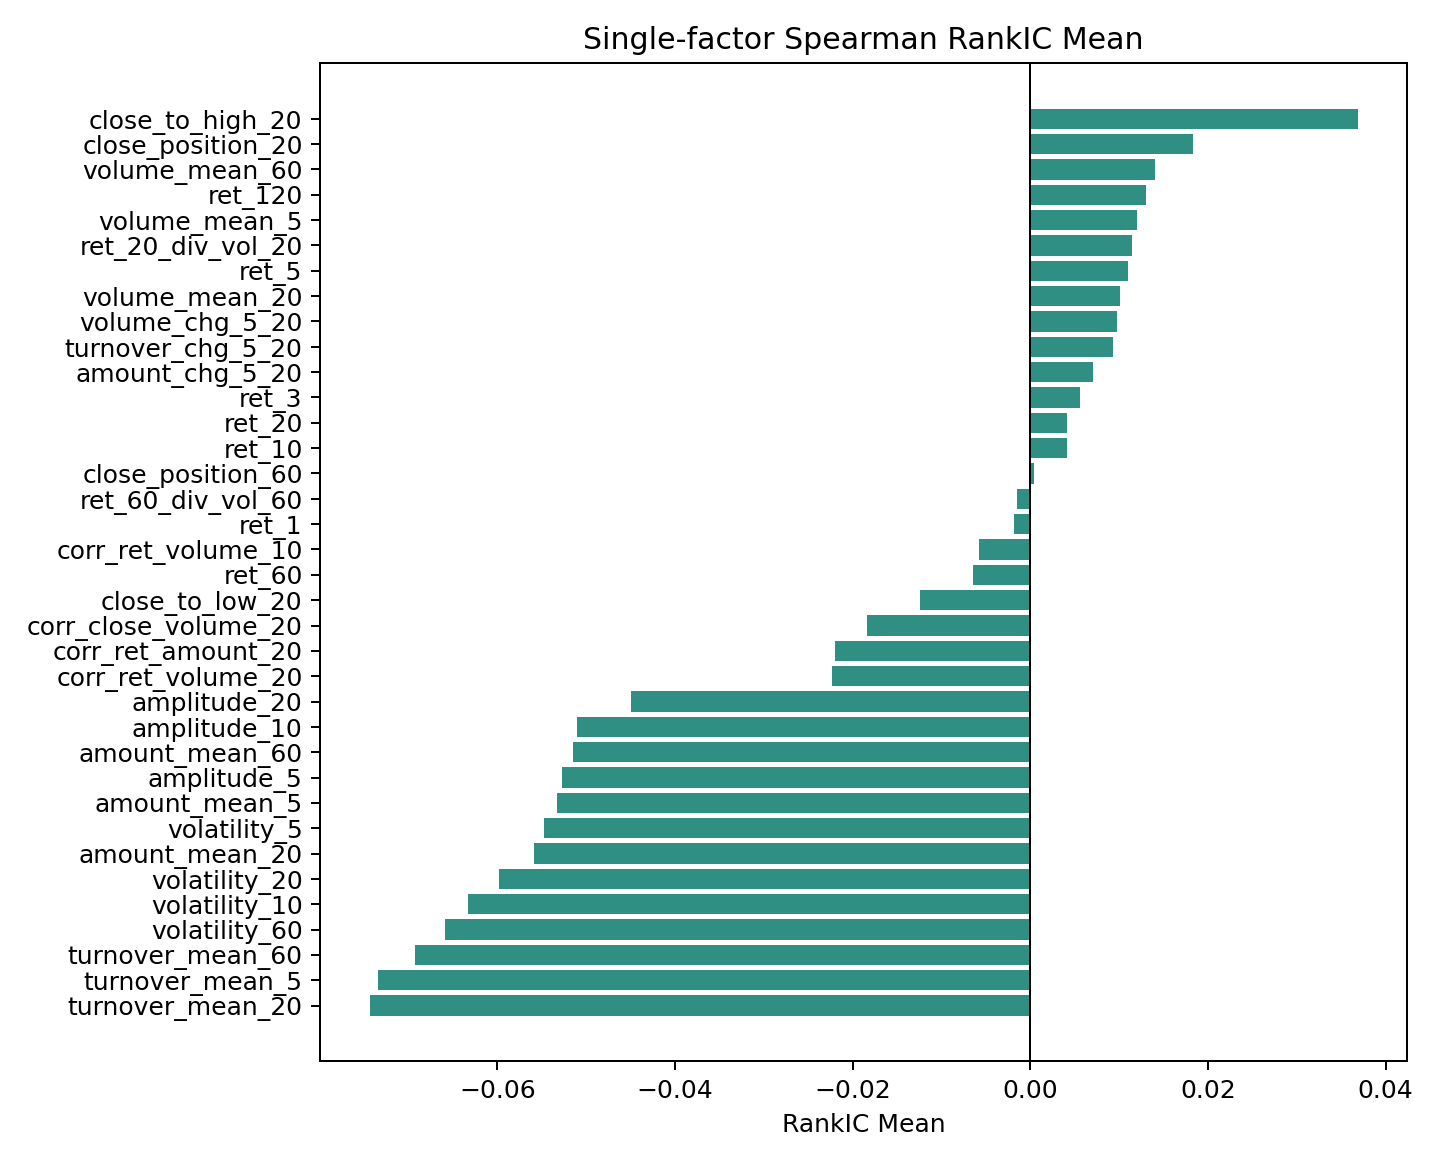
\includegraphics[width=\linewidth]{figures/factor_rankic_bar.png}
\caption{单因子 RankIC 均值}
\end{figure}

\begin{figure}[H]
\centering
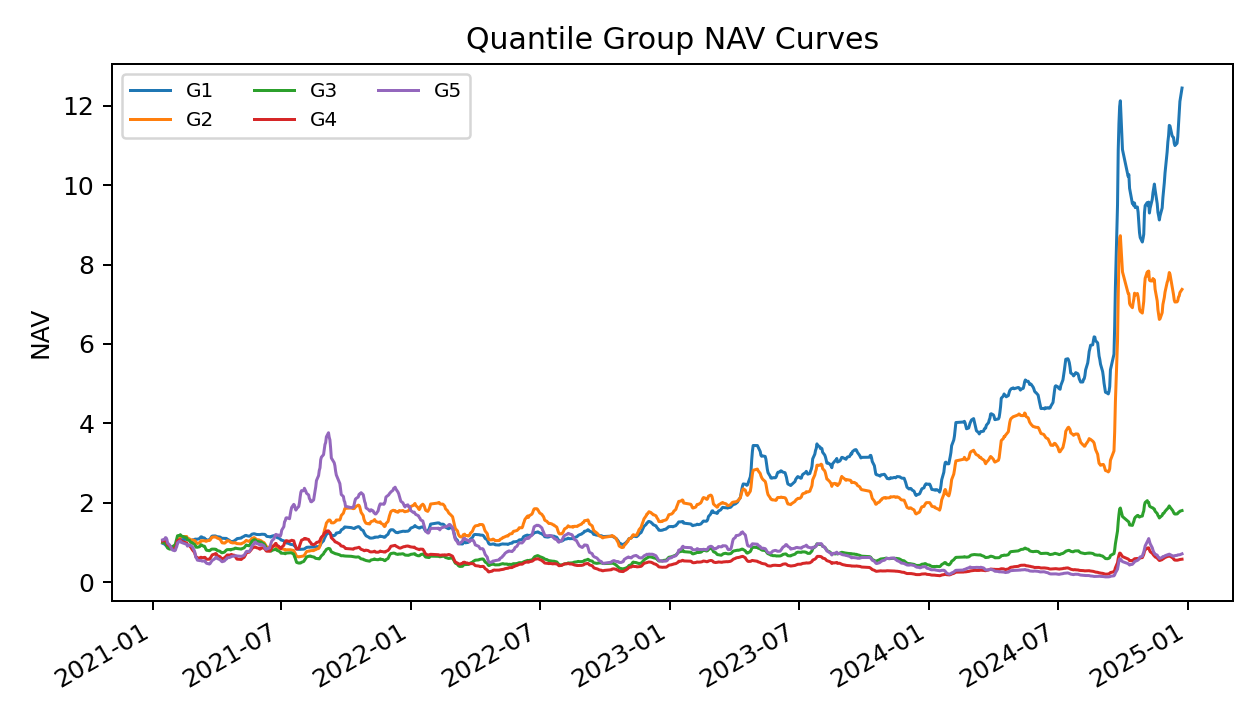
\includegraphics[width=\linewidth]{figures/group_nav_curve.png}
\caption{最高 RankIC 因子的分组净值曲线}
\end{figure}

\section{Machine Learning Models}
Random Forest 作为 bagging-based nonlinear benchmark，用于检验普通非线性树模型是否能捕捉因子关系 \cite{breiman2001random}。XGBoost 是经典 boosting tree model，适合建模非线性和因子交互 \cite{chen2016xgboost}。LightGBM 是本文主力 GBDT 模型，适合较大规模 tabular panel data \cite{ke2017lightgbm}。PyTorch MLP 是 simple deep learning baseline，结构为 128/64 hidden units、BatchNorm、ReLU 和 Dropout。

本文不将 MLP 或更复杂深度模型视为天然更优。日频价量因子通常噪声高、样本有效信息有限，MLP 容易过拟合，且缺少树模型对 tabular 特征切分的归纳偏置。因此模型比较重点放在样本外 RankIC、分组收益和交易成本后表现，而非训练集拟合误差。

\begin{table}[H]
\centering
\caption{样本外预测指标（AKShare test set）}
\resizebox{\linewidth}{!}{\begin{tabular}{lllll}
\toprule
Model & MSE & $R^2$ & Daily IC & Daily RankIC \\
\midrule
Random Forest & 0.0037 & -0.0042 & 0.0385 & 0.0258 \\
XGBoost & 0.0037 & -0.0082 & 0.0305 & 0.0208 \\
LightGBM & 0.0038 & -0.0162 & 0.0252 & 0.0245 \\
MLP & 0.0037 & -0.0123 & 0.0304 & 0.0430 \\
\bottomrule
\end{tabular}
}
\end{table}

\section{Backtesting Framework}
回测规则为每 5 个交易日调仓一次，在调仓日 $t$ 使用模型预测分数，选择分数最高的前 10\% 股票，于 $t+1$ 开始等权持有 5 个交易日。benchmark 为股票池等权组合。默认单边交易成本为 10 bps，并额外测试 5、10、20 bps。评价指标包括年化收益、年化波动率、Sharpe、最大回撤、换手率和交易成本后收益。

\section{Empirical Results}
样本按时间切分：训练集为 2021-07-05 至 2023-08-01，验证集为 2023-08-02 至 2024-04-15，测试集为 2024-04-16 至 2024-12-23。表 \ref{tab:backtest} 展示 AKShare 测试集下的模型回测结果。等权 benchmark 的测试期年化收益为 0.3176；模型多头组合在该测试期没有稳定跑赢 benchmark，说明弱正 RankIC 不一定转化为交易成本后的超额收益。

\begin{table}[H]
\centering
\caption{模型回测指标（10 bps，AKShare test set）}
\label{tab:backtest}
\resizebox{\linewidth}{!}{\begin{tabular}{llllll}
\toprule
Model & Annual Return & Annual Vol & Sharpe & Max DD & Turnover \\
\midrule
Random Forest & 0.2978 & 0.3461 & 0.9111 & -0.1754 & 1.0353 \\
XGBoost & 0.2381 & 0.3135 & 0.8264 & -0.1574 & 1.0647 \\
LightGBM & 0.1523 & 0.3160 & 0.5947 & -0.1872 & 1.0941 \\
MLP & 0.2956 & 0.1820 & 1.5133 & -0.0846 & 1.1882 \\
\bottomrule
\end{tabular}
}
\end{table}

\begin{figure}[H]
\centering
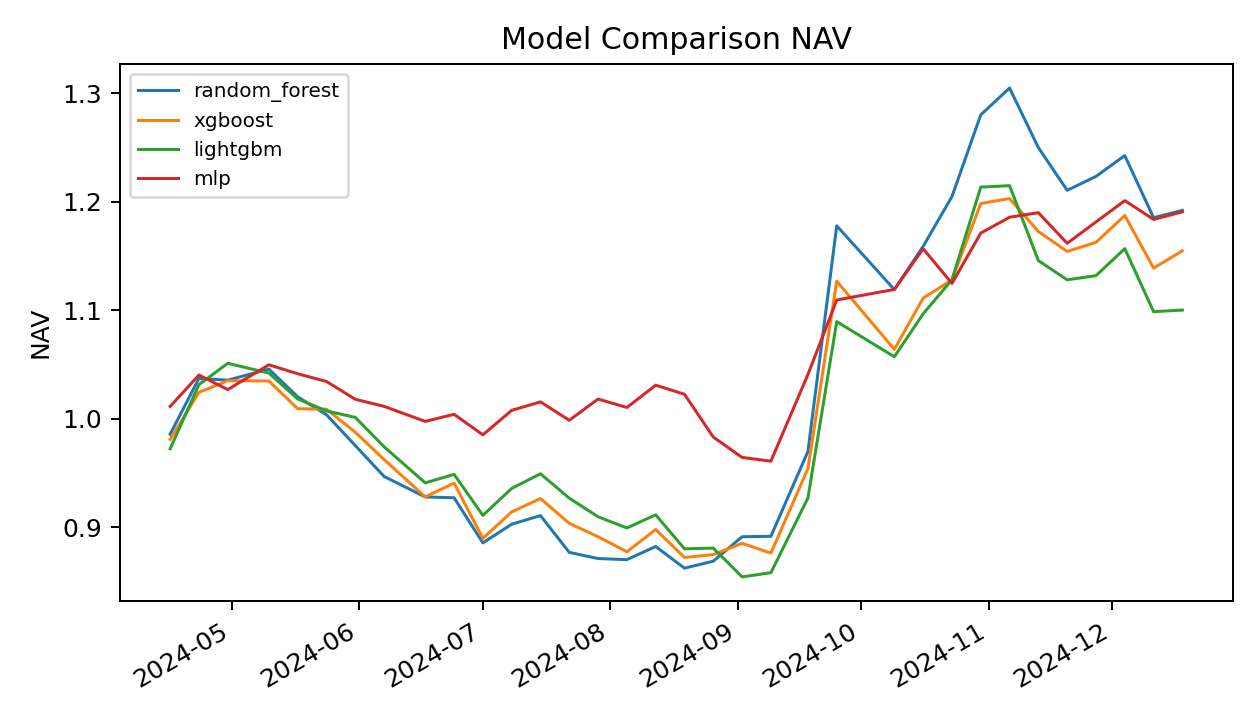
\includegraphics[width=\linewidth]{figures/model_comparison_nav.png}
\caption{不同模型净值对比}
\end{figure}

可以看到，所有模型的样本外 $R^2$ 均为负，但 RankIC 为弱正。这符合金融收益预测常见现象：点预测解释度很低并不必然否定横截面排序信息，但排序信息也不必然足以形成可交易超额收益。因此评价模型时，需要同时观察 RankIC、分组收益、交易成本后净值、换手和回撤。

\section{Robustness Checks}
稳健性分析覆盖不同交易成本、不同持有期和不同模型。交易成本上升会压缩净收益，说明组合换手和成本控制是 Alpha 能否落地的重要环节。

\begin{table}[H]
\centering
\caption{交易成本敏感性（LightGBM score，AKShare test set）}
\resizebox{\linewidth}{!}{\begin{tabular}{lllll}
\toprule
Cost bps & Annual Return & Sharpe & Max DD & Turnover \\
\midrule
5.0000 & 0.1846 & 0.6825 & -0.1793 & 1.0941 \\
10.0000 & 0.1523 & 0.5947 & -0.1872 & 1.0941 \\
20.0000 & 0.0904 & 0.4195 & -0.2029 & 1.0941 \\
\bottomrule
\end{tabular}
}
\end{table}

\begin{figure}[H]
\centering
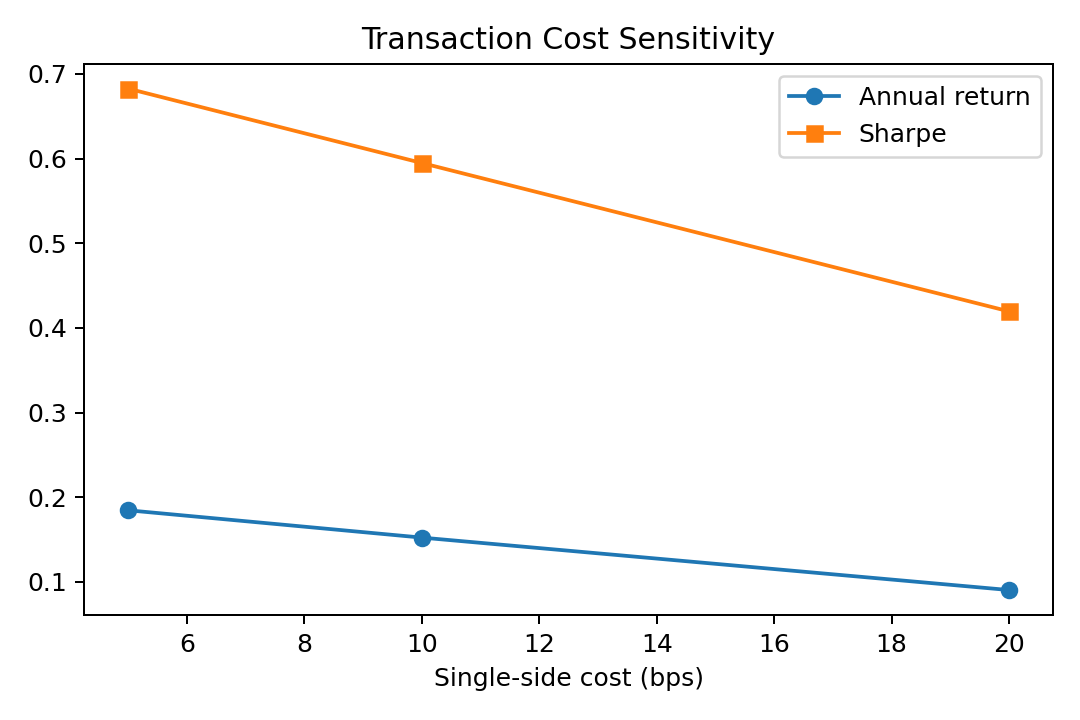
\includegraphics[width=\linewidth]{figures/cost_sensitivity.png}
\caption{交易成本敏感性}
\end{figure}

\begin{table}[H]
\centering
\caption{持有期稳健性（LightGBM score，AKShare test set）}
\resizebox{\linewidth}{!}{\begin{tabular}{lllll}
\toprule
Horizon & Annual Return & Sharpe & Max DD & Turnover \\
\midrule
1d & 0.0704 & 0.3687 & -0.2015 & 0.6840 \\
5d & 0.1523 & 0.5947 & -0.1872 & 1.0941 \\
10d & 0.3763 & 1.2149 & -0.1467 & 1.3412 \\
20d & 0.4515 & 1.0652 & -0.1528 & 1.4500 \\
\bottomrule
\end{tabular}
}
\end{table}

\section{Avoiding Look-ahead Bias}
本项目从以下方面控制未来信息泄露。第一，所有因子只使用 $t$ 日及以前数据；第二，标签从 $t+1$ 开始计算，避免用当日无法成交的价格；第三，rolling 特征按股票分组并使用历史窗口；第四，去极值和标准化均在每个日期横截面内独立完成；第五，模型训练只使用过去数据预测未来数据；第六，不使用随机 train\_test\_split；第七，不使用缺少公告日期的财务数据；第八，固定股票池可能存在幸存者偏差；第九，测试集仅用于最终评估。

\section{Limitations and Future Work}
本文局限包括：AKShare 公共接口可能不稳定或字段变化；固定示例股票池不等于完整全 A point-in-time 股票池；交易成本假设简化，未考虑市场冲击成本；未加入真实高频订单簿；未进行严格行业中性化；未处理全部涨跌停、停牌和 ST 约束；未加入实盘验证；MLP 可能过拟合。后续可扩展至 point-in-time A 股真实数据、行业风险模型、组合优化、涨跌停约束、高频 LOB 特征、Temporal CNN 或 Transformer，但前提是数据口径和验证框架足够严格。

\section{Conclusion}
本文完成了一个从 AKShare 数据到因子、从模型到回测、从样本外验证到报告展示的 Machine Learning Alpha Research 框架。本次结果没有被包装成稳定盈利策略，而是展示了更真实的量化研究结论：机器学习模型可以提取弱排序信号，但交易成本、benchmark、换手和稳健性决定其是否具有进一步研究价值。

\bibliographystyle{plain}
\bibliography{references}

\end{document}
